\section{Pre-processing}
The data is pre-processed in MatLab to prepare it to the three different neural network models. Each model has an appurtenant data representation which are prepared in three different ways. The three data representations are morphology, regions and superimposed morphology and region. Common for the data representation is that the pain maps are imported as image-matrices whereafter the matrices are resized, since the given data was collected at different resolutions (screen sizes). Furthermore, the matrices are cropped to sort out unnecessary data like the areas inferior and superior to the knee.
Before the data is used as an input in the neural network models, the image-matrices are converted into vectors whereafter they are assembled in one matrix for each data representation. To get additional information associated with the pain maps, is gender added by including a column vector to the three matrices. 
In addition to the input, the neural network models need an output to train the models. The output, which is either symptom duration or pain intensity, is likewise added as a column vector. 
The following sections describe the pre-processing of the individual data representations. 

\subsection{Morphology} \label{sec:Morph}
The first representation of data is a binary matrix of the original pain maps.
Firstly, the image of the original pain map is gray-scaled to get a one-dimensional matrix instead of a three-dimensional RGB-matrix. This matrix is then converted into a matrix consisting of zeroes and ones, where the pain pixels are symbolized with ones. An original pain map and a pain map consisting of a binary matrix is shown in figure \ref{fig:cropbin7}.

\begin{figure} [H]
\centering
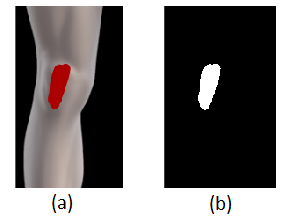
\includegraphics[width=0.7\textwidth]{figures/cropbin7}
\caption{(a) Original pain map and (b) image consisting of a binary matrix where white color represents the pain pixels.}
\label{fig:cropbin7}
\end{figure}

\noindent
An illustration of this data representation is created to convey how the data is assembled and transferred to the model. The illustration is shown in figure \ref{fig:binmatrix}.

\begin{figure} [H]
\centering
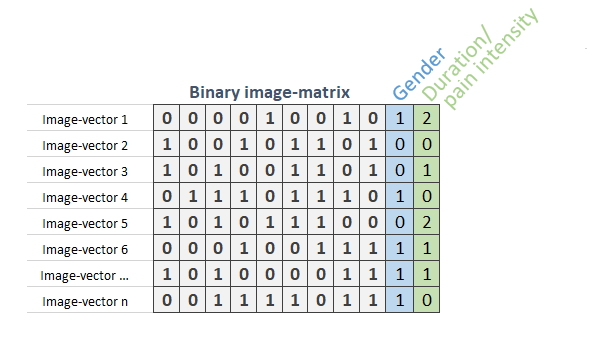
\includegraphics[width=0.8\textwidth]{figures/binaryimagematrix}
\caption{An illustration of the matrix of the morphology data representation. The matrix consist of image-vectors for each subjects where the two last column indicate the appurtenant gender and either duration or pain intensity. The image-vectors has a length equal to the number of pixel in the pain maps.}
\label{fig:binmatrix}
\end{figure}


\subsection{Regions}
The second representation of the data is a matrix consisting of vectors with 20 values which indicate pain in relation to the knee regions.
The knee regions shown in figure \ref{fig:atlas} are converted into a matrix consisting of 20 values, which represent each knee regions. This matrix is superimposed to the binary image of the pain map, which results in a matrix with pain represented in each knee region. In figure \ref{fig:binregions} are the knee regions and the pain associated with the regions illustrated.

\begin{figure} [H]
\centering
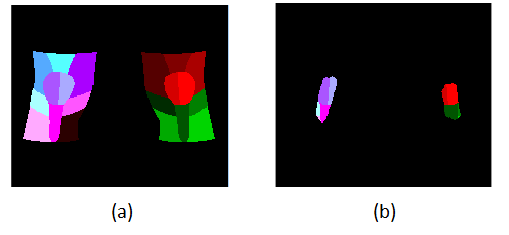
\includegraphics[width=0.8\textwidth]{figures/binregions}
\caption{(a) Knee regions and (b) pain in the specific regions.}
\label{fig:binregions}
\end{figure}

\noindent
After superimposing the two matrices, knee regions and pain, the number of pixels in each active knee region is found. This number is compared to the total number of pixels that are in each knee region, so knee regions with less than 15 \% pain are excluded. WHY 15\%. As a result a vector with 20 values is created. This data representation is implemented the same way as the first representation, figure \ref{fig:binmatrix}. The only difference is that the length of the image-vectors respond to the 20 regions, and therefore are there only 20 values in this data representation.


\subsection{Superimposed morphology and regions}
The third representation of the data is a matrix consisting of individuals’ pain divided into the knee regions.
\noindent
In this representation the superimposed matrix from the second data representation is used. Since the data representation should reflect the morphology of the pain and divide the pain into the different knee regions is one-hot encoding used. One-hot encoding is a way to separate categorical data into binary data \citep{Harris2012}. This means that the 20 values for each knee region do not have a correlation. After one-hot encoding the superimposed matrix consists of 20 layers where each layer represents a knee region. An illustration of this data representation is shown in figure \ref{fig:onehot}.


\begin{figure} [H]
\centering
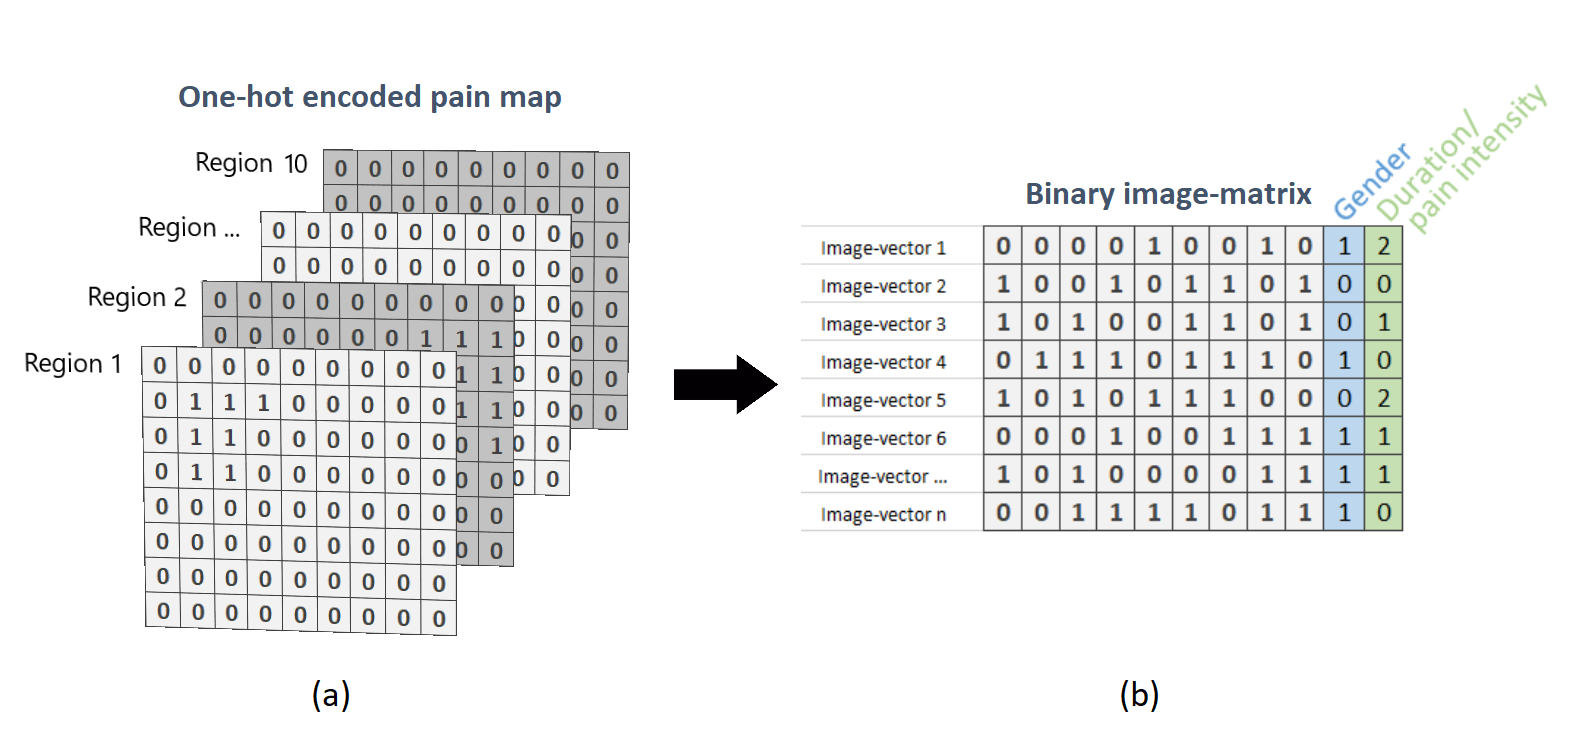
\includegraphics[width=1\textwidth]{figures/onehotmatrix}
\caption{(a) illstrates the one-hot encoded pain map and (b) shows the images-vectors in one assembled matrix with gender and either symptom duration or pain intensity.}
\label{fig:onehot}
\end{figure}